\documentclass[tikz,border=2pt]{standalone}
\usepackage{amsmath,amssymb}
\usepackage{tikz}
\usetikzlibrary{arrows.meta}

\begin{document}
% Every polynomial of degree n >= 1 has exactly n complex roots counted with multiplicity:
% z^5 - 1 has the five fifth roots of unity, only one of them real.
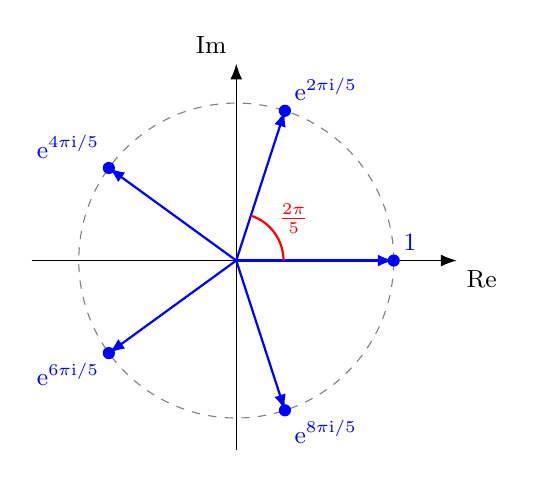
\begin{tikzpicture}[every node/.style={font=\small}, >={Latex[length=2mm]}]
	\draw[->] (-2.6,0) -- (2.8,0) node[below right] {$\mathrm{Re}$};
	\draw[->] (0,-2.4) -- (0,2.5) node[above left] {$\mathrm{Im}$};
	\draw[gray, dashed] (0,0) circle (2);
	\foreach \k in {0,1,2,3,4} {
		\draw[blue, thick, ->] (0,0) -- ({72*\k}:2);
		\fill[blue] ({72*\k}:2) circle (2.2pt);
	}
	\node[blue, above right] at (0:2) {$1$};
	\node[blue, above right] at (72:2) {$\mathrm{e}^{2\pi \mathrm{i}/5}$};
	\node[blue, above left] at (144:2) {$\mathrm{e}^{4\pi \mathrm{i}/5}$};
	\node[blue, below left] at (216:2) {$\mathrm{e}^{6\pi \mathrm{i}/5}$};
	\node[blue, below right] at (288:2) {$\mathrm{e}^{8\pi \mathrm{i}/5}$};
	\draw[red, thick] (0.6,0) arc (0:72:0.6);
	\node[red, font=\small] at (36:0.9) {$\tfrac{2\pi}5$};
\end{tikzpicture}
\end{document}
